% Ubah judul dan label berikut sesuai dengan yang diinginkan.
\section{Literature Review}
\label{sec:relatedworks}

\subsection{Electric Wheelchair}
A wheelchair is a manually operated or power-driven device designed primarily for use by individuals with mobility disabilities for the primary purpose of moving indoors, or indoors and outdoors.  Individuals with mobility disabilities must be permitted to use wheelchairs and manually powered mobility aids, such as walkers, crutches, canes, or other similar devices designed for use by individuals with mobility disabilities, in any area open to pedestrian traffic \cite{ADA_2023}. An electric wheelchair can be seen in Figure \ref{fig:kursiroda}.

%Gambar 2.1
% Contoh input gambar
\begin{figure}[ht]
  \centering

  % Ubah dengan nama file gambar dan ukuran yang akan digunakan
  \includegraphics[scale=0.2]{gambar/bab3/wheel.jpeg}

  % Ubah dengan keterangan gambar yang diinginkan
  \caption{Electric Wheelchair}
  \label{fig:kursiroda}
\end{figure}

\subsection{Eye Gesture}

Eye gesture refers to eye movements, such as eye gaze, eye pose, and facial expressions, which play an important role in human communication and interaction. Eye tracking devices have been used to study various aspects of eye pose, including the influence of social factors, physical factors, and the relationship between eye pose and speech. These devices can record participants' eye poses with a corneal reflex camera and analyze body pose and eye pose with temporal accuracy \cite{gullberg_kita_2009}. An example of an eye pose can be seen in Figure \ref{fig:gaze}.

% Gambar 2.2
\begin{figure} [ht] \centering
    % Nama dari file gambar yang diinputkan
    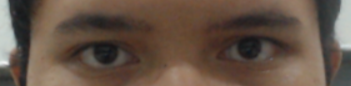
\includegraphics[scale=0.5]{gambar/bab3/gaze.png}
    % Keterangan gambar yang diinputkan
    \caption{Eye Pose}
    % Label referensi dari gambar yang diinputkan
    \label{fig:gaze}
\end{figure}

\subsection{MediaPipe Face Mesh}

MediaPipe Face Mesh is a face landmark detection solution that estimates 468 3D face landmarks in real-time, even on mobile devices. The solution utilizes a pipeline of two neural networks to identify 3D coordinates of facial landmarks from 2D images. The first network, BlazeFace, calculates the location of the face from the full image, while the second network operates on the cropped region to identify the location of the landmarks \cite{mediapipe_2020}. The technology has a wide range of applications, including face mask detection, hands-free computer control, and gestures accompanying speech \cite{thaman_2022}. A visualization of the MediaPipe Face Mesh can be seen in Figure \ref{fig:facemesh}.

% Gambar 2.3
\begin{figure} [ht] \centering
    % Nama dari file gambar yang diinputkan
    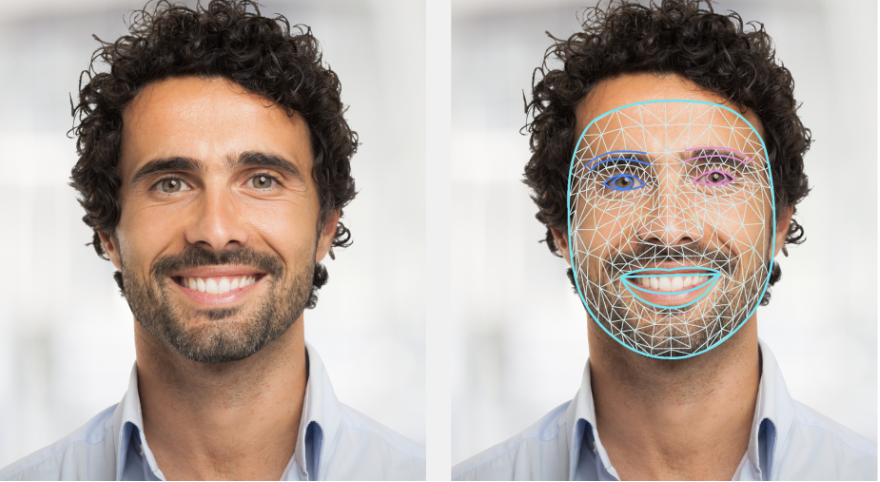
\includegraphics[scale=0.4]{gambar/face_landmark.png}
    % Keterangan gambar yang diinputkan
    \caption{MediaPipe Face Mesh}
    % Label referensi dari gambar yang diinputkan
    \label{fig:facemesh}
\end{figure}

\subsection{Convolutional Neural Network (CNN)}

A Convolutional Neural Network (CNN) is a type of artificial neural network used primarily for image recognition and processing. It is a subset of machine learning and is specifically designed to identify and recognize objects in images, as well as for tasks such as object classification and pattern recognition \cite{arm_2023}. 

The architecture of a CNN consists of three parts, namely input, feature learning, and classification. The Feature Learning consists of two convolution layers and two pooling layers. In classification consists of two hidden layers and one output layer. CNN architecture can be depicted as in Figure \ref{fig:arsitektur cnn}.

% Gambar 2.4
\begin{figure} [ht] \centering
    % Nama dari file gambar yang diinputkan
    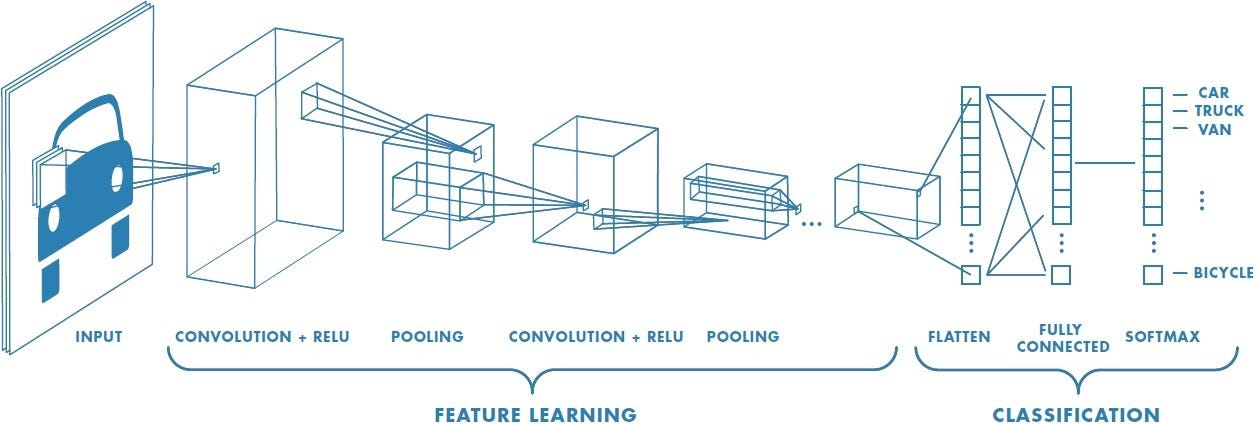
\includegraphics[scale=0.2]{gambar/cnn.jpg}
    % Keterangan gambar yang diinputkan
    \caption{Convolutional Neural Network Architecture}
    % Label referensi dari gambar yang diinputkan
    \label{fig:arsitektur cnn}
\end{figure}

\subsection{Confusion Matrix}

The Confusion Matrix is a tool used to evaluate the performance of classification models in machine learning. It provides a detailed overview of how the classification model works, showing the relationship between the model's predictions and the actual values. The Confusion Matrix is a tabular representation consisting of four main components, namely True Positive (TP), False Positive (FP), True Negative (TN), and False Negative (FN). Each component has a specific meaning in the context of prediction \cite{provost2013data}. The visualization of confusion matrix can be seen in Figure \ref{fig:confusion}.

% Gambar 2.7
\begin{figure} [ht] \centering
    % Nama dari file gambar yang diinputkan
    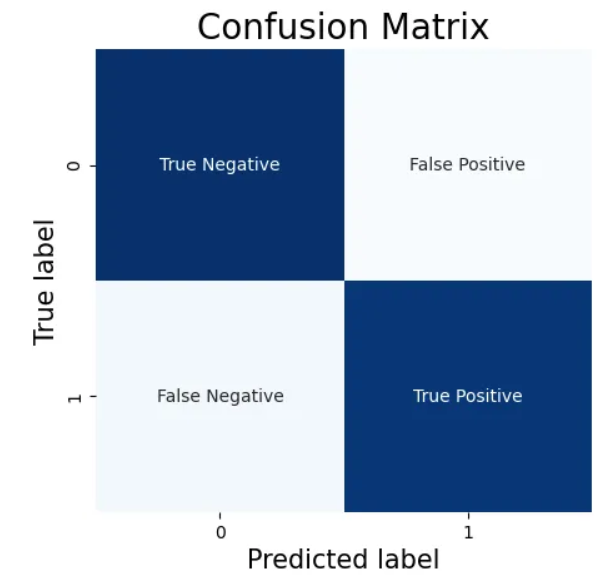
\includegraphics[scale=0.3]{gambar/bab2/confusion.png}
    % Keterangan gambar yang diinputkan
    \caption{Confusion Matrix Visualization}
    % Label referensi dari gambar yang diinputkan
    \label{fig:confusion}
\end{figure}

\subsection{Accuracy}
\label{subsec:acc_klasifikasi}

Accuracy is a performance measure that indicates how correctly the model can classify the test data. In this context, accuracy is the ratio of correct predictions (TP and TN) to the total amount of data. In other words, accuracy measures how close the predicted value is to the actual value. The value of accuracy can be obtained using Equation \ref{eq:acc}.

\begin{equation}
  \label{eq:acc}
  Accuracy=\frac{TP+TN}{TP+TN+FP+FN}
\end{equation}

\subsection{Precision}
\label{subsec:prec_klasifikasi}

Precision is a performance measure that indicates the degree of accuracy of the requested data compared to the predicted results provided by the model. In this context, precision is the ratio of correct positive predictions (TP) to the total positive prediction results (TP and FP). The value of precision can be obtained by Equation \ref{eq:prec}.

\begin{equation}
  \label{eq:prec}
  Precision=\frac{TP}{TP+FP}
\end{equation}

\subsection{Recall}
\label{subsec:recall_klasifikasi}

Recall is a performance measure that indicates how successful the model is in retrieving information. In this context, recall is the ratio between correct positive predictions (TP) and the total number of positive actual data (TP and FN). Thus, the recall value can be calculated using Equation \ref{eq:recall}.

\begin{equation}
  \label{eq:recall}
  Recall=\frac{TP}{TP+FN}
\end{equation}

\subsection{F1-Score}
\label{subsec:score_klasifikasi}

The F1-Score is a value between zero (0) to one (1) obtained from the harmonic mean between the precision value and the recall value. Therefore, the value of F1-Score can be calculated using Equation \ref{eq:score}.

\begin{equation}
  \label{eq:score}
  F{1}{-}Score=\frac{2 \times Precision \times Recall}{Precision+Recall}
\end{equation}

\subsection{Next Unit of Computing (NUC)}

Intel NUC, or Next Unit of Computing, is a mini computer device that has high computing power in a compact form. With its small dimensions, NUC is still able to provide powerful performance for various computing needs. The latest NUC models are equipped with the latest generation of Intel Core processors, support 4K graphics, and have extensive connectivity capabilities such as Thunderbolt, USB, HDMI, and Ethernet. These advantages make it an ideal choice for edge computing applications and applications that require high computing power in a limited space \cite{intel_nuc}.